\chapter{Lösungsansatz}
\label{ch:S4_Lösungsansatz}

\section{Mögliche Lösungen}
\label{ch4:s:Lösungen}

\subsection*{Gamification}


Im Hinblick auf die Problemstellung in Kapitel \ref{ch2:Problemstellunug}, sowie der in der Literatur beschriebenen Ansätze in Kapitel \ref{ch3:s:Gamification}, ergeben sich mehrere Möglichkeiten für eine Lösung. Ziel ist es die Kunden zum einen zu motivieren neue Geschäfte aufzusuchen und auf der anderen Seite eine Bindung zu bestehenden Geschäften zu erreichen. Da es sich hierbei um um einen Prozess handelt, der für den Kunden im ersten Schritt nur einen geringen Benefit darstellt, ist dieser ideal für Gamification geeignet \cite{Leigh.2012}. Ziel ist es somit die Besuche des Spielers durch eine Gamification interessant zu machen. Dies kann durch die verschiedenen Aspekte wie das Vergeben von Punkten für einen Einkauf (siehe Miles \& More \cite{Wagner.2005}, Payback \cite{Roesl.2005}) erreicht werden. Allerdings sind reine, einfache Punkteprogramme weit verbreitet und deren Nutzen umstritten \cite{Schmitt.2001}.
Daher ist es notwendig, das komplette Spektrum der Gamification zu betrachten.
Über das reine Punkte System hinaus, manifestiert sich in der Literatur die Grundmenge "Points, Badges und Leaderboards".
Konkret bedeutet dies, neben der einfachen Ansammlung von Punkten, gibt es darüber hinaus Badges/Auszeichnungen welche das Engagement des einzelnen Nutzers widerspiegeln. Ein weiterer Aspekt sind die sogenannten Leaderboards bzw. Bestenlisten. Über diese wird wird ein Ansporn unter den jeweiligen Spielern erzeugt die anderen Spieler zu übertrumpfen. Vergleicht man diese Ansätze mit denen der typischen Spieler Profile nach \citep{Bartle.2004}, wie in Abbildung \ref{img:ch4_img01_playertypes} zu sehen, so erkennt man, dass nicht alle dieser mit den Standard Elementen bedient werden.

\begin{figure}[H]
\begin{center}
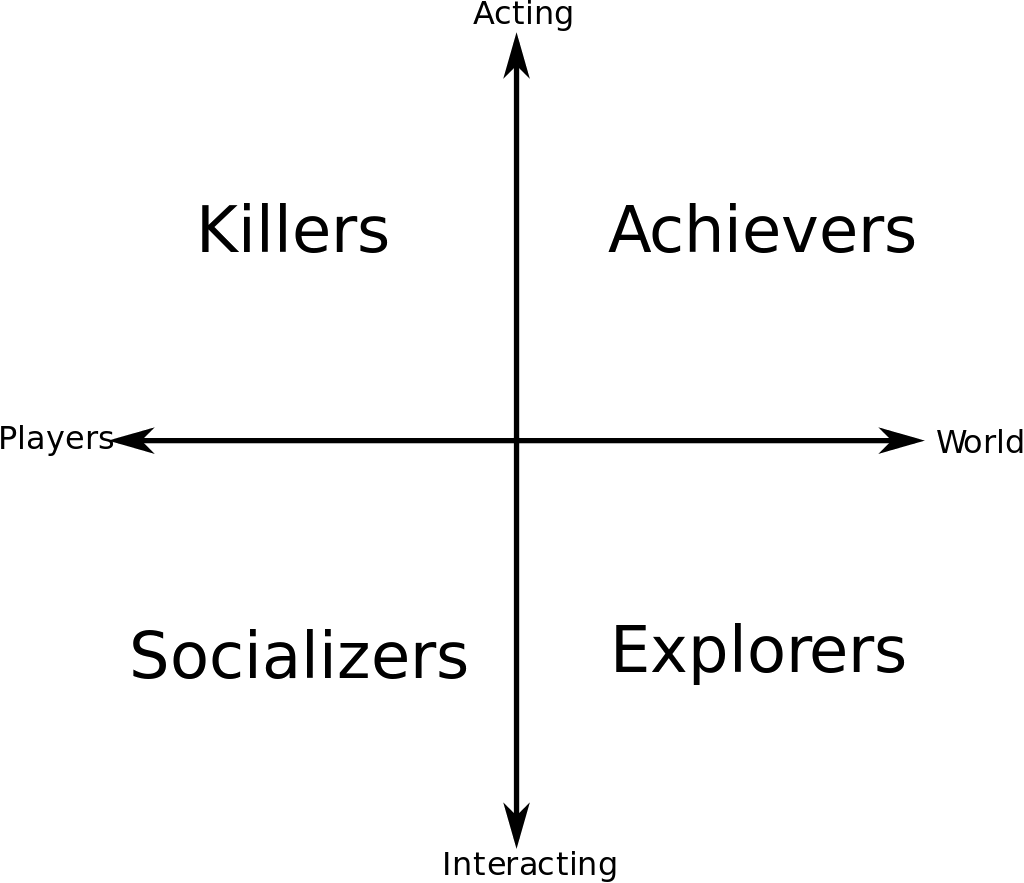
\includegraphics[width=120mm]{images/ch4_img01_playertypes.png}
\caption{Spielertypen nach \textcite{Bartle.2004}}
\label{img:ch4_img01_playertypes}
\end{center}
\end{figure}

Die rudimentären Elemente der Gamification richten sich vor allem an Achievers und Killers.
Die Frage stellt sich hierbei, wie Socializers und Explorers erreicht werden können.
Hierzu kann das von \cite{Zichermann.2011} in Kapitel \ref{ch3:s:Gamification} erweiterte Modell SAPS genutzt werden, welches auch auf die Interaktion unter den Menschen eingeht. Im konkreten Beispiel schlägt Zichermann vor, den Spielern die Möglichkeit zu geben bestimmte Positionen innerhalb eines Spiels einzunehmen. Durch diese sollen einzelne Spieler eine höhere Position erhalten als andere und damit auch eine Interaktion untereinander fördern. Damit kann können zumindest zu einem gewissen Teil die Socializers abgedeckt werden.
Es ist jedoch zu beachten, dass für die vollständige Abdeckung aller Spielertypen konkret eine Spielmechanik erarbeitet werden muss, welche die übrigen zwei Spielertypen explizit bedient. Möglichkeiten sind hierbei eine Interaktion zwischen den Spielern zu schaffen, stellen z.B. das Erstellen von Teams/Gilden dar, welche gemeinsam aktiv handeln. Gemeinsame Ziele können so einfacher verfolgt werden aber auch speziell durch das Spiel ein Zusammenhalt explizit gefördert werden. Dies kann z.B. anhand von Bonuspunkten oder aber von Handlungen die explizit die Interaktion von mehreren Spielern erfordern. Ein Beispiel hierfür ist das Spiel Ingress von Google welches für die Erstellung von Portalen im späteren Spiel umso mehr Spieler benötigt, je höher dessen Level sein soll. \cite{Celino.2013}
Andere Ansätze sind kooperative Quests, Handel von Spielitems, sowie das Fördern von Kommunikation zwischen den einzelnen Spielern. \cite{Caon.2013} Ein weiterer Aspekt sind neue Bekanntschaften, die durch ortsbezogene Spiele gemacht werden. In einer Umfrage von 6400 Ingress Spielern gaben 84\% an neue Leute kennen gelernt zu haben und zählten dies zu einem wichtigen Faktor des Spiels \cite{Ingress.2014}.
Explorer untersuchen Ihre Umgebung und möchten neue Dinge entdecken. Sie fragen nach zusätzlichen Informationen. Für diese Spieler ist es z.B. interssant n neue unbekannte Orte innerhalb des Spiels zu gelangen.

Dass die einzelnen Spielertypen nicht zu vernachlässigen sind wird in \cite{Bromley.2013} deutlich. Hierbei stellt der Autor am Beispiel von GoPets fest, dass durch die Orientierung an konkrete Spielertypen ein beachtliche Umsatzsteigerung erzielt werden kann. \cite{Bethke.2007} Allerdings ist es wichtig für den Erfolg eines Spieles, dass alle Spielertypen adressiert werden.
\\\\
Nachdem die (Spiel-)Elemente der Gamification selbst identifiziert wurden, muss untersucht werden, wie die Interaktion der Spieler mit dem lokalen Einzelhandel aussehen kann.
Der Unterschied des Einzelhandels im Vergleich zum Onlinehandel ist der geografische bzw. physikalische Besuch. Der Kunde muss physikalisch vor Ort sein, um eine Dienstleistung wahrzunehmen oder aber ein Produkt zu kaufen. Daher ist es für den jeweiligen Händler von besonderem Interesse, dass ein potentieller Kunde sein Geschäft betritt.
Ziel ist es somit den Spieler durch die Spielmechanik in das jeweilige Geschäft zu bringen.
Hierbei gibt es zwei Mögliche Ansätze für ein ortsbezogenes Spiel. In der ersten und einfachsten Möglichkeit tritt das Geschäft selbst als festes Spielelement auf, dass direkt zum Spielerfolg beiträgt. In diesem Fall repräsentiert das Geschäft zum Beispiel ein TicTacToe Feld. Eine andere Möglichkeit ist es die Spieler indirekt zu unterstützten. In diesem Fall tritt das Geschäft z.B. als virtueller laden im Spiel auf, über den die Spieler entsprechende Items kaufen können.
Welche der beiden Möglichkeiten in Frage kommt, hängt von der Intention des einzelnen Händlers ab. Steht der Fokus des Spiels auf einem reinen Kontakt mit dem Spielelement, so 
muss sicher gestellt werden, dass die Spieler nicht einfach nur den jeweiligen Laden einfach nur betreten und dann wieder direkt verlassen. Im schlimmsten Fall kann dies sogar dazu führen, dass normale Kunden die nicht am Spiel selbst teilnehmen sich durch die Spieler gestört fühlen.
Da es hierfür keinerlei Erwartungswerte gibt, ist der Aspekt schwer abzuschätzen, allerdings wäre eine mögliche Gegenmaßenahme, die Verweildauer der Spieler zu erhöhen, in dem Sie z.B. ein kleines Rätsel lösen müssen oder für eine gewisse Zeit im entsprechenden Raum aufhalten müssen.
Des weiteren kann dem Händler auch die Möglichkeit gegeben werden, wiederkehrende Spieler bevorzugt zu behandeln. Ein Konzept welche z.B. bei Foursquare verwendet wird ist der Mayor einer Location. Der Mayor stellt dabei die Person,da welche die Lokalität innerhalb der letzten 60 Tage am häufigsten besucht hat. Diesem kann ein Händler über Foursquare besonderes Angebot machen, wie zum Beispiel ein Kaffee zum halben Preis.\cite{Lindqvist.2011} Ähnliche Konzepte können hier analog ebenfalls verwenden werden.
\\\\
Da das Hauptaugenmerk darauf liegt, dass der Spieler mit dem jeweiligen Geschäft interagiert, muss sichergestellt werden, dass dieser physikalisch vor Ort ist. 
Um dies sicherzustellen, gibt es mehre Möglichkeiten. Die einfachste Variante ist es einfach die GPS-Koordinaten des Systems zu verwenden. Der Vorteil liegt darin, dass bei den meisten mobilen Betriebssystemen eine A-GPS Implementierung vorliegt, die die Nachteile von reinem GPS unter Zuhilfenahme einer bestehenden Mobilfunkverbindung kompensiert \cite{Djuknic.2001}. Allerdings könnte es sein, dass der Empfang ein einzelnen Gebäuden eingeschränkt ist und weder eine Verbindung zu GPS-Satelliten noch zum Mobilfunknetz hergestellt werden kann. Darüber hinaus besteht die Problematik, dass die Genauigkeit nicht ausreicht um festzustellen, ob die Person vor dem Geschäft oder im Geschäft selbst ist.
Es muss daher sichergestellt werden, dass der Spieler wirklich im Geschäft selbst ist.
Hier zu könnte man QR-Code verwenden die entsprechend abgescannt werden und darüber eine Interaktion über eine URL oder App iniitiert werden. Eine andere neue Möglichkeit stellt NFC dar \cite{Rashid.2006b}. Über diese kann im Bereich von bis zu 20cm eine Interaktion stattfinden. \cite{Coulton.2006} passive NFC Elemente arbeiten in diesem zusammenhang analog zu QR Codes was den Datenaustausch angeht. Der Unterschied liegt darin, dass die Daten nicht per Kamera sondern per NFC erfasst werden. Diese Ansätze breiten sich aktuell im Handel immer mehr aus \cite{Heinemann.2014}. In Seoul gibt es z.b. virtuelle Stores, bei denen es sich um Werbeposterflächen handelt, die ein Regal mit QR-Code darstellen \cite{Tesco.2012}. Diese werden vor allem in besonders gerne während des Feierarbendverkehrs genutzt.
Eine neue Technologie die neben den QR-Codes und NFC zum Einsatz kommen könnte sind Bluetooth Low Energy Devices (BLE). Apple setzt bereits diese in den Appstores ein und einige Startups sehen in der Technologie eine Möglichkeit den lokalen Einzelhandel mit dem Online Geschäft zu verbinden. Konkret handelt es sich dabei um passive BLE Geräte welche bis zu 30 Meter haben können und deren Entfernung über eine Approximierung von RSSI und der übermittelten Referenzsignalstärke angegeben wird. \cite{Do.2013} Durch den Einsatz von mehreren sogenannter Beacons kann analog zur GPS Lateration eine Indoor Positionierung erreicht werden.\footnote{Ein entsprechendes System wurde vom Autor entwickelt und evaluiert} Somit könnte der konkrete Aufenthaltsort in einem speziellen Bereich z.B. der Herrenmode belohnt werden.
\\\\
Ein Aspekt der nicht außer Acht gelassen werden darf, ist dass bei Spielen, bei denen es darum geht mit anderen Spielern verglichen zu werden, immer zwangsläufig zum Cheating kommt. \textcite{Consalvo.2005} Ein besonderer Augenmerk gilt hier dem Multiplayer Cheating. Dabei geht es konkret um eine Vorteilsnahme gegenüber den anderen teilnehmenden Spielern.
\textcite{Yan.2005} identifiziert mehrere Möglichkeiten des Cheatings. Für diese gibt es jeweils entsprechende Gegenmaßnahmen. Als Grundsatz kristallisiert sich daher heraus, dass der Schutz eines Spiels analog zum investierten Aufwand gegen entsprechende Versuche der Manipulation verhält und dass kein System sicher gegen eine Manipulation ist.
Jeder Spielebetreiber muss basierenden auf seinen verfügbaren Resourcen entscheiden, welche Methoden dieser einsetzten möchte. 
Auch ortsbezogene Spiele bleiben von Manipulationen nicht verschont wie \textcite{He.2011} untersucht.
In diesem Fall ist ein erster Ansatzpunkt die maximale Fortbewegungsgeschwindigkeit. Kombiniert man diese mit der Spielmechanik wie z.b. einer Pflicht Interaktiondauer von 30 Sekunden pro POI, so reduziert sich auch der "Vorteil" durch das Cheaten.

%
\subsection*{Anforderungen an ein Geogameframework}

Für die Umsetzung eines Geogameframeworks muss zunächst untersucht werden welche Anforderungen an ein solches gestellt werden.
Im Hinblick auf die in Kapitel \ref{ch2:Problemstellunug} beschriebene Problemstellung ist es zunächst sinnvoll die Anforderungen zu identifizieren und im Anschluss zu analysieren. Werden diese Abstrahiert auf die Aspekte eines Gameframeworks so ergeben sich daraus entsprechende Vorgehensweisen.
\\\\
Ziel ist es ein ortbezogenes Spiel zu entwickeln, welches dazu führt, dass die Spieler lokale Dienstleister/Einzelhändler vermehrt aufsuchen. Ein Gameframework muss in diesem Fall einem Spielleiter es ermöglichen unter möglichst wenig Aufwand ein entsprechendes Spiel durchzuführen.
Dem Spielleiter sollen die Arbeitsschritte für die Selektion der Spielelemente anhand von  Geodaten als auch die Durchführung abgenommen werden. Ziel ist es, dass der Spielleiter selbst mit möglichst geringen Technischen Kenntnissen ein entsprechendes Spiel durchführen kann. Daher halten wir als ersten Aspekt das einfache Staging der Spiele fest.
\\\\
Für die Steigerung der Interaktion von potentieller Kunden wurde die Gamification und letztendlich die konkrete Spielemechanik in Kpaitel \ref{ch3:s:Gamification} identifiziert. Um diese entsprechend umsetzten zu können, muss ein entsprechendes Framework nicht nur entsprechende Logik, sondern auch die entsprechenden Daten inne halten. Abhängig wie hoch der Flexibilitäts Anspruch des Frameworks selbst ist, macht es Sinn Spiel-Logik und Spiel-Daten weiter zu trennen. Soll das Framework nur für eine geringe Zahl ähnlicher Spiele verwendet werden, so kann es Sinn machen die Funktionen und Datenstruktur direkt in das Framework einzuplanen. Ist es allerdings der Plan ein Framework zu entwickeln, welches möglichst generisch arbeitet und später eine Vielzahl an unterschiedlichen Spielen unterstützten soll, so ist eine entsprechende Modularisierung der einzelnen Funktionen unerlässlich.
\\\\
Bei der Durchführung eines ortsbezogenen Spiels muss ein Framework mit Geodaten arbeiten.
Dabei ist es unerlässlich, dass ein entsprechendes System nicht mit einem einfachen kartesischen Koordinaten System arbeitet, sondern ein entsprechendes Referenzsystem wie WGS 84 \cite{Grafarend.1998} und das UTM Koordinaten System \cite{Grafarend.1995}.
Für das jeweilige zu nutzende System müssen entsprechende Bibliotheken integriert werden, damit entsprechende Operationen wie zum Beispiel Distanzmessung auf den Geodaten durchgeführt werden können.
\\\\
Das Framework muss zudem die Integration vom externen GeoDaten ermöglichen. Bei diesen wird es sich Aufgrund der Ergebnisse in Kapitel \ref{ch3:s:offeneGeodaten} um OSM handeln. Das Framework muss auf Basis der OSM Daten entsprechende Spielfelder aufbereiten. Hierzu müssen die bestehenden Objekttypen (Nodes, Ways, Relatitoions) in Spielelemente transferiert werden. Hierfür gibt es mehrere Möglichkeiten.
Zunächst gibt es Nodes. Diese können direkt als Spielelement dargestellt werden, da Sie analog zu den Spielelementen ein Objekt repräsentieren und ihnen eine direkte Koordinate auf dem Spielfeld zugeordnet werden kann. Nodes die jedoch Bestandteil eines Ways oder einer Relation sind sollten nicht als einzelnes Spielelement betrachtet werden.
Gibt es ein Objekt, welches als Way oder Relation in OSM repräsentiert wird, so muss dieses zu einem Spielement mit nur einer Koordinate transformiert werden. Hierzu müssen alle Nodes welche innerhalb eines Ways liegen zu einem "virtuellen" Node zusammengefasst werden.
Wichtig ist hierbei eine Adressierung der virtuellen Nodes zu ermöglichen. Damit diese entsprechend wieder gefunden werden können.
Für die Transformation mehrere Nodes zu einem Element gibt es unterschiedliche Ansätze. Der erste und einfachste stellt ein einfaches Arithmetisches Mittel auf die äußersten Kanten des Ways dar. Konkret bedeutet das, dass um alle Nodes eines Ways quasi eine Bounding Box gebaut wird. Die beiden Koordinaten die die Bounding Box begrenzen werden anschließend mit einem arithmetischen Mittel miteinander kombiniert zu einem einzelnen Punkt. Diese Methode ist besonders einfach und der Punkt liegt immer innerhalb der Bounding Box, allerdings spiegelt er nicht die Verteilung der einzelnen Objekte wieder bzw. nimmt auf die konkrete geografische Struktur des Ways keine Rücksicht:

\begin{equation}
x_{bb} = \frac{max_{i>0; i<=N}(x_i) + min_{i>0; i<=N}(x_i)}{2}
\end{equation}
\\
\begin{equation}
y_{bb} = \frac{max_{i>0; i<=N}(y_i) + min_{y>0; i<=N}(y_i)}{2}
\end{equation}

Eine weitere Methode die diese Unzulänglichkeit behebt stellt der geometrische Schwerpunkt dar.
Bei diesem wird der Massenmittelpunkt des Körpers bestimmt\cite{Papula.2006}. Hierfür ist zunächst die Berechnung der Fläche nötig:

\begin{equation}
A = \frac{1}{2}\sum_{i=0}^{N-1} (x_i\ y_{i+1} - x_{i+1}\ y_i)
\end{equation}

Dieses kann wiederum verwendet werden um das geometrische Gewicht zu ermitteln:

\begin{equation}
x_s = \frac{1}{6A}\sum_{i=0}^{N-1}(x_i+x_{i+1})(x_i\ y_{i+1} - x_{i+1}\ y_i)
\end{equation}

\begin{equation}
y_s = \frac{1}{6A}\sum_{i=0}^{N-1}(y_i+y_{i+1})(x_i\ y_{i+1} - x_{i+1}\ y_i)
\end{equation}

Die jeweiligen x- und y-Koordinaten liefern damit die entsprechenden Koordinaten auf dem Spielfeld.
\\\\
Der Gedanke eines Frameworks zielt auf eine einfache Erweiterbarkeit, Pflege sowie Wiederverwendbarkeit ab. Daher ist die Erweiterbarkeit für weitere Spiele und Spielmechaniken ein wichtiger Aspekt. Ziel ist es daher ein Grundgerüst zu entwickeln, welches durch entsprechende Anpassung einfach angepasst werden kann.
Je nach Fokus auf Flexibilität, welche das Framework bieten soll und Umfang, müssen entsprechende Funktionen und Methoden generischer oder spezifischer implementiert werden.
\\\\
Der in Kapitel \ref{ch1:Einleitung} angestrebte Mehrwert des Frameworks, neue Kunden und bestehende Kunden an lokale Einzelhändler zu binden stellt ein wichtiger Aspekt dar. Generell gibt es verschiedene Möglichkeiten wie Lokalitäten in ein Spiel integriert werden können \cite{Nelson.2002}.
Zunächst gibt es die Möglichkeit Werbebanner direkt in Spiele einzubinden \cite{Nelson.2004}. Diese Werbung gleicht der Printwerbung mit dem Unterschied, dass die Sichtbarkeit im Vergleich zu klassischen Medien oder Filmen deutlich erhöht ist und und sich analog zur durchschnittlichen Spielzeit verhält. Spiele die soziale Aspekte betrachten, haben im Schnitt höhere Spielzeiten \cite{Ducheneaut.2006}, bei älteren Spielern sind bis zu 30 Stunden pro Spiel der Durchschnitt.

Eine andere Möglichkeit stellen so genannte Advergames dar. Bei diesen handelt es sich um Spiele die rein auf dem zu bewerbenden Produkt bzw. der Dienstleistung selbst fokusiert sind. Diese haben einen deutlich größeren Einfluss auf die entsprechende Zielgruppe. Allerdings werden hierbei vor allem Personen angesprochen die Spielen gegenüber offen sind \cite{Winkler.2006}. \textcite{Chen.2001} und \textcite{Dahl.2009} beschreiben, dass jüngere Personen bis zu 100 mal mehr spielen als ältere und der Kunde die Marke durch Advertgames deutlich mehr wahrnimmt im Vergleich zu anderer Werbung.
Die Möglichkeiten für die Integration von Produkten sind vielfältig. Neben der passiven Einbindung des Produktes in die Spielumgebung, kann das Produkt auch selbst als Spielelement dienen (vgl. Colgate 1992: Harald Hårtand -- kampen om de rene tænder).
Darüber hinaus könnte im Fall eines ortsbezogenen Spieles der Händler/Dienstleister im Spiel selbst als Pendant seines Händlers in der Realität auftreten. D.h. ein Händler stellt im Spiel selbst einen Händler für Spielitems dar.
Somit lässt sich die Einbindung generell in zwei Arten unterteilen. Einmal als aktiv für den Spielausgang entscheidendes Element (z.B: als POI für TicTacToe) oder aber als Vendor Element welches der Spieler aufsuchen kann.
Im Hinblick auf die Spieleitems sollten diese vorzugsweise im Zusammenhang mit dem Händler und der Spielthematik stehen. Je besser sich diese in das Spiel integrieren, desto eher werden sie vom Spieler als plausibel wahrgenommen. Dies wiederum hat einen positiven Effekt für die Wahrnehmung.
Ein Beispiel für die Integration könnte z.B. ein Supermarkt sein, welcher Essen anbietet. Dieses kann wiederum vom Spieler zur Auffrischung der Energie verwendet werden. Ein anderes Item könnte eine Schaufel darstellen, welche beim lokalen Baumarkt gekauft und im Spiel zum Bauen von eigenen Gebäuden verwendet werden kann.
\\\\
Abschließend muss das Framework entsprechend modular aufgebaut werden sein. Dies soll vor allem der Erweiterbarkeit und der Portabilität dienen. Da ein ortsbezogenes Spiel auf entsprechenden Endgeräten gespielt wird. Konkrekt Smartphones ist es darüber hinaus wichtig entsprechend die Spielelemente für den Spieler aufzubereiten. Hierzu gibt es verschiedene Möglichkeiten.
Generell gibt es unterschiedliche Smartphone Betriebssysteme deren Marktanteile sich je nach Geografischer Location unterscheiden.
Schaut man sich die globale aktuelle Verteilung der mobilen Betriebssysteme an, wie in Abbildung \ref{img:ch4_img02_marketshare} zu sehen.

\begin{figure}[H]
\begin{center}
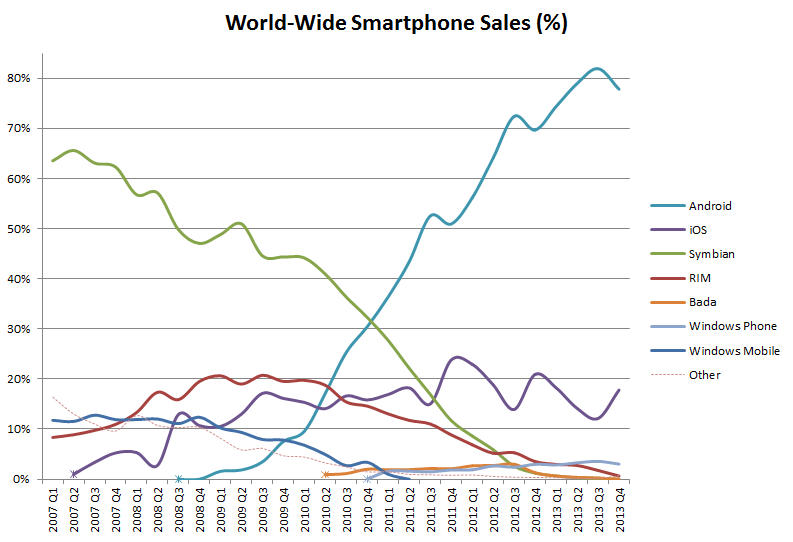
\includegraphics[width=140mm]{images/ch4_img02_marketshare.png}
\caption{Globale Mobile Betriebsysteme in Anlehnung an \textcite{Gartner.2013} -- Bild: \cite{Wikipedia.2014}}
\label{img:ch4_img02_marketshare}
\end{center}
\end{figure}

Die aktuelle Verbreitung von ca. 80\% Android, 18\% iOS und 3\% Windows Phone bei Smartphones stellt die Frage, für welche der besagten Plattformen man Anwendungen erstellen möchte.
Die erste Möglichkeit sind native Apps, zweitere sind Web App \cite{Charland.2011}.
Der Unterschied beider liegt im Aufwand der Implementierung, der Ausführgeschwindigkeit, Zugriff auf die Hardware und dem unterschiedlichen Deployment.
Native Apps erreichen in den entsprechenden Appstores und bieten Zugriff auf allerlei Hardware Features.
Konkret für das Geogameframework sind zweierlei Dinge wichtig.

\begin{itemize}
\item Möglichst wenig Aufwand für das Deployment
\item Zugriff auf GPS Korrdinaten
\end{itemize}

Dies kann sowohl über native  Apps als auch über eine Web Applikation bewerkstelligt werden. Entsprechende SDKs der jeweiligen Hersteller bieten per API Zugriff auf die GPS Schnittstelle. Für WebApps kann im Zuge von HTML5 ebenfalls auf eine GPS Ortung zurückgegriffen werden \cite{Holdener.2011}. Um den Entwicklungsaufwand für Webapps zu reduzieren kann es sinnvoll sein auf entsprechende Webframeworks aufzusetzten, damit nicht grundlegende Funktionalitäten erneut entwickelt werden müssen.
Eine entsprechende Entscheidung ist in diesem Fall abhängig von den Anforderungen. Eine entsprechende Auswahl wird in Kapitel \ref{ch:S5_Umsetzung} getroffen.

Abschließend lassen sich die einzelnen Anforderungen des Gameframeworks wiefolgt zusammenfassen:

\begin{itemize}
\item einfaches Staging der Spiele
\item Modularisierung der Funktionen für Gamification/Spielmechanik
\item Verarbeitung von Geodaten
\item OSM-Daten Transformation/Aufbereitung
\item Einfache Erweiterbarkeit der Spielmechanik
\item Einbindung der lokalen Händlern
\item Modularer Aufbau
\end{itemize}


\subsection*{Relokalisierbarkeit von ortsbezogenen Spielen}

Für die Relokalisierbarkeit von Spiefeldern wurden in Kapitel \ref{ch3:s:Relokalisierung} erste Ansätze in der Literatur identifiziert. Diese beziehen sich allerdings speziell auf spatial discrete Spiele.
Generell erfolgt die Unterteilung in die zuvor identifizierten Möglichkeiten.
Es kann entweder keine Anpassung, eine vollständige Anpassung oder ein Hybrid Ansatz erfolgen. Der ideale Fall stellt eine vollständige Anpassung und damit Relokalisierbarkeit eines Spiels ohne das manuelle Anpassen eines Spielleiters dar. Hier für gibt es in der Literatur allerdings keine konkreten Ansätze. Vielmehr werden konkrete Spiele wie REXplorer \cite{Ballagas.2007} oder bestimmte Geogames \cite{Kiefer.2007} adaptiert durch eine vorgegebene Liste an POIs zu einem optimalen Spielfeld in einer anderen Stadt von der ebenfalls eine Liste von POIs existiert.
Einen evaluierten nutzbaren Ansatz für die automatisierte Relokalisierung gibt es daher nicht.
Ein Ansatz der sich aus der Hypothese herausbildet, ist der Versuch Aufgrund bestehender Geodatenbanken -- konkret Openstreetmaps -- eine Relokalisierung zu erreichen. Hierbei müssen allerdings neben der bereits angesprochenen Transformation der Relationen, Ways und Nodes auch eine Auswahl der entsprechenden Spielelemente stattfinden. Denkbar sind hierbei zwei Ansätze. Um ein "gutes Spielfeld" zu identifizieren und somit eine Relokalisierung für gut zu befinden muss entsprechend ein Evaluationsansatz existieren. Ansätze zur Evaluation von Spielfeldern sollen im Kapitel \ref{ch:S6_Evaluierung} näher betrachtet werden. Generell kann zwischen einer Echtzeit und einer prestaging Evalutation unterschieden werden. Je Form hat ihre eigenen Vor- und Nachteile.

Bei einer Echzeitevaluation der Spielfelder liegt der Vorteil in völligen Automatisierung der Auswahl der Spielelemente und weniger Aufwand für den entsprechenden der ein Spiel ausrichten möchte. Allerdings muss gleichzeitig der zu verwendende Algorithmus in Echtzeit zu einem entsprechenden Ergebnis für die Auswahl der Spielelemente kommen. Da die ortbezogenen Pervasive Games selbst in Echtzeit laufen kann ein entsprechender Algorithmus keine größere Komplexität aufweisen und wird damit in der möglichen Qualität der Spielfelder eingeschränkt.

Im Gegensatz dazu steht eine Evaluation und Auswahl der Spielelemente vor dem Staging. Die Vorteile sind die mögliche Komplexität des Algorithmus, sowie die damit verbundene Qualität der Spielfelder. Ein Nachteil ist allerdings, dass eine Evaluation der Spielfelder im Voraus erfolgen muss. Da bei einem Pervasive Game allerdings das Spielfeld die ganze Welt darstellt, ist eine Laufzeit stark abhängig vom Algorithmus sowie der Datenbasis.

Eine andere Möglichkeit stellt ein hybrider Ansatz dar. Dabei wird ein Teil des Evaluation vorausgelagert und ein weniger komplexer Teil für die Echzeitberechnung übrig. Eine Möglichkeit wäre es z.B. Im Voraus eine Selektion der Spielelementtypen und die konkrete Auswahl in diesem Subset an Daten während der Laufzeit zu machen. Beispielsweise mit OSM könnte im Voraus zunächst eine Auswahl der Kategorisierung anhand eines key-value Paars erfolgen (highway=bustop) und im Anschluss wird während der Laufzeit entschieden ob entsprechende Objekte zu dicht beieinander liegen. Dann könnten die Elemente entsprechend außer acht gelassen werden oder bei zu geringer Verbreitung entsprechende dummy-Elemente eingefügt werden.

\subsection*{Freie Geobasisdaten und Möglichkeiten der kommerziellen Nutzung}

In Kapitel \ref{ch3:s:offeneGeodaten} wurden entsprechende öffentliche Geodatenbanken identifiziert welche Geodaten enthalten, die für eine Nutzung für ein ortsbezogenes Spiel in Frage kommen. Von diesen hat sich lediglich OSM als brauchbar und mit entsprechender Daten-Qualität erwiesen. Untersucht man Openstreetmap bezüglich seiner Lizenz für die Verwendung in kommerziellen Projekten, so lässt sich zunächst der Wechsel der Lizenz im Jahre 2012 auf ODbl erkennen \cite{Ramthun.2012}.

Vergleicht man die Anforderungen eines Gameframeworks an die entsprechenden Geodaten so ist der Punkt wichtig, dass im Vergleich mit anderen Open Source Lizenzen eine Kommerzielle Nutzung möglich ist, ohne den Quellcode des Programmes oder zusätzlicher externen Datenquellen selbst zu veröffentlichen.
Die OBdl in Version 1.0 \cite{Odbl.2014} beschreibt hierbei, dass ein Auszug aus der Datenbank selbst als Derivative Database anzusehen ist. D.h. konkret in Verbindung mit OSM, dass das Ergebnis einer Abfrage an den OSM Server als Datenbank anzusehen ist, welche nach Odbl zu behandeln ist. Der Nutzer, hier: Betreiber, ist verpflichtet, wenn die OSM Daten selbst modifiziert werden oder in irgend einer Weise aufgewertet/aufbereitet und der Öffentlichkeit (über das Internet) zur Verfügung gestellt werden, diese ebenfalls öffentlich zu machen. Eine private Verwendung muss nicht veröffentlicht werden. Gleiches gilt für die zusätzlichen externen Datenquellen welche mit den OSM Daten vermengt werden. Dies können zum Beispiel kommerziell eingekaufte Höhenprofile oder Landschaftsaufnahmen sein. Diese bleiben somit davon unberüht.

Vergleicht man nun die Pflichten die durch die Nutzung der ODbl in Verbindung mit OSM entstehen mit den Anforderungen des Gameframeworks, so lässt sich feststellen, dass eine Nutzung der OSM Daten juristisch unbedenklich ist, allerdings die abgerufenen Daten über eine dokumentierte Schnittstelle wieder zur Verfügung gestellt werden sollten.
Wie eine Dokumentation und zur Verfügungsstellung der Daten im Detail aussieht ist nicht näher spezifiziert. Hier eignet es sich eine bestehende Schnittstelle, welche im Entwurf de Frameworks geplant ist entsprechend so zu erweitern, dass diese entsprechend die Daten zur Verfügung stellt. Idealerweise stellt dies eine Schnittstelle dar, die analog zur Datenaufbereitung für das Spielfeld dient. Alternativ könnte man, um die Performance des Spiels nicht zu beeinträchtigen auch einen separaten kleineren Server dafür abstellen, welcher die gleiche Funktionen bietet, aber verhindert, dass durch die Abfrage von größeren Datenmengen nicht das laufende Spiel beeinträchtigt wird.

\section{Gewählter Lösungsansatz}
\label{ch4:s:choosen_solution}

Betrachtet man die in Kapitel \ref{ch1:Einleitung} beschriebene Forschungsfrage, so ist der Fokus der Arbeit vor allem auf der Untersuchung einer Möglichkeit zur möglichst einfachen Aufbereitung von Spielfelder zu sehen, bei denen der Spielveranstalter so wenig wie möglich sich selbst einbringen muss. Darüber hinaus sollen die lokalen Händler/Dienstleister in das Spiel eingebunden werden, damit diese entsprechend einen Mehrwert durch Kundenbindung erfahren.
Da der Fokus auf die Aufbereitung und Evaluation der Spielfelder gelegt wurde, werden für das Beispielspiel nur ein teil der Aspekte umgesetzt.

Für die Gamification selbst ist es nach Analyse der Möglichkeiten am sinnvollsten sich überwiegend auf die Basis Elemente Points Badges und Leaderboards zu beschränken. Spätere Elemente die \textcite{Zichermann.2011} herausgearbeitet haben, sollten entsprechend einfach erweiterbar sein, aber nicht den Fokus darstellen. Um die einzelnen Aspekte besser zu verdeutlichen, werden die verwendeten Aspekte am Beispielspiel erläutert.
\\\\
Das Beispielspiel selbst stellt eine abgewandelte Variante des beliebten Capture The FlagSpielmodus \cite{Atkin.1999}.
Es gibt verschiedene Flaggen auf dem Spielfeld. Diese Flaggen symbolisieren entsprechende POIs, welche auf Basis des Gameframeworks unter der Nutzung von OSM generiert wurden. Dem Spieler stehen entsprechende Aktionspunkte zur Verfügung, welche er einsetzten kann um diese Flaggen zu besetzten. Jeder eingesetzte Aktionspunkt, führt zu "Prestige" auf der Flagge. Der Spieler kann Flaggen, welche von fremden Spielern bereits besetzt wurden übernehmen, in dem er diese durch den Einsatz seiner Aktionspunkte um deren Prestige verringert bis diese neutral sind. Neutrale Flaggen kann der Spieler wiederum einnehmen. Dem Spieler stehen pro Tag 24 Aktionspunkte zur Verfügung. Jede Stunde erhält der Spieler einen Aktionspunkt, sofern er noch nicht mindestens 24 Aktionspunkte hat. Durch Den Kauf von Items über Händler unter dem Einsatz Aktionspunkte, kann der Spieler seine Fähigkeiten verbessern. Der aktuelle Punktestand, welcher sich aus dem Prestige aller Flaggen die dem Spieler angehören berechnet, ist dem Spieler ersichtlich. Über diesen hinaus kann sich der Spieler mit Spielern aus seiner geografischen Nähe, sowie seinen Mitspielern in der Rangliste unter und über ihm messen.
\\\\
Die Wahl für ein der Spielmechanik nach unkompliziertes Spiel fiel, da der Fokus auf der Generierung der Geodaten bzw. Spielelemente lagt und darüber hinaus durch die Repräsentation der Spielelemente durch einfache POIs die Verwendung des Geogameframeworks generisch genug ist um sowohl für Pervasive Games als auch für Geogames eingesetzt werden zu können. Die Spielmechanik, welche an Capture the Flag erinnert, ist besonders beliebt bei Spielern und hat sich auch in bestehenden Pervasive Games bewährt \cite{Bell.2006,Ingress.2014}. Darüberhinaus erfüllt es in der genannten Abwandlung bereits einige Aspekte der Gamification Elemente. So wird der Status des Spielers bzw. sein "Prestige" direkt anhand der Flaggen auf dem Spiefeld sichtbar. Er kann sich auch mit anderen Spielern messen und seine Interaktion mit dem Spiefeld wird für die anderen Spieler direkt in Echtzeit ersichtlich.
Die Einführung der Aktionspunkte für die Interaktion mit der Umgebung hat zwei Intentionen. Zum einen soll sichergestellt werden, dass die ortsbezogenen Affordanzen für die einzelnen Spieler normalisiert werden. Hiermit wird versucht ein quasi Handicap für besonders aktive und sich schnell fortbewegenende Spieler zu erstellen. Es wird darüber hinaus verhindert, dass der Spieler sich nur kurz in bestimmten Regionen aufhält und das Spiel somit nicht zu einem Rennspiel sich ausbildet \cite{Schlieder.2005}. Ein weiterer Nebeneffekt ist die Reduzierung von möglichen Betrugsversuchen, da selbst eine Automatisierung der Spielerclients durch z.B. Bots keinen entscheidenden Vorteil bringt \cite{Golle.2005}. Durch die Limitierung der Aktionspunkte auf 24 pro Tag wird der Spieler nichtsdestotrotz animiert jeden Tag im Spiel aktiv zu sein, da ansonsten seine Aktionen "verfallen". Items, welche der Spieler von Händlern kaufen kann, sollen als Gegenstand dem Spieler repräsentiert werden, der nicht nur einfach beim Händler kaufbar und dann im Inventar verwendbar ist, sondern auch mit anderen Spielern teilbar. Die Idee dahinter spielt auf die beliebten Rollenspiel Elemente ab und soll dazu dienen, dass Spieler miteinander z.B. durch Handeln physikalisch interagieren. Speziell die Spielertypen Socializer werden hier angesprochen. Aber auch Explorer kommen hier zum Zug, da die Items bzw. Itemtypen nicht starr festgelegt sind und somit jede REgion oder jeder Händler individuelle Items besitzen kann. Die Händler/Dienstleister selbst werden hier als nicht gewinnbringendes Spielelement aktiv. Die Entscheidung dass die Händler nicht selbst als POIs auftreten, auf die eine Flagge gesetzt werden kann hat zwei Überlegungen. Zum einen sollen die Händler nicht von Spielern "besetzt" werden, damit keine Assoziation zwischen "Besitz" der Händler stattfindet, zum anderen soll eine gewisse Modularisierung stattfinden. D.h. sofern sich die Bedingungen bzw. die Auswahl der POIs verändert, können die Händler unabhängig vom generierten Spielfeld am Spielteilnehmen. Somit kann das Framework auch in einem anderen Zusammenhang verwendet werden und es kann darüber hinaus eine feine Selektion der teilnehmenden Händlern stattfinden.
Die Integration eines entsprechenden Leaderboards ermöglicht den Spielern sich mit geografischen und punkte nahen Spielern zu messen. Dies ist vor allem für die Spielertypen Achiever und Killer relevant. Letztere wird darüber hinaus die Möglichkeit gegeben gezielt Spielern zu schaden, wenn sie explizit Flaggen eines bestimmten Spielers angreifen.
\\\\
Für die Anforderungen des Geogameframeworks wurde entschieden, dass zunächst das Framework dazu eingesetzt werden soll um entsprechende  Spielfelder zu generieren, unabhängig des darauf aufbauenden Spieles. Das Beispielspiel wird somit als Proof of Concept des darunterliegenden Frameworks agieren. Es soll ein entsprechendes Webframework verwendet werden, welches die Daten über eine entsprechende Schnittstelle dem Spiel zur Verfügung stellt und damit bestehende Technologien nutzt um den Implementierungsaufwand auf das Framework zu konzentrieren und nicht auf die Tools für die Konfiguration und Darstellung. Für die Basis der Geodaten wird auf OSM zurückgegriffen werden, und die damit verbundenen Lizenzanforderung der Verfügbarkeit der verwendeten Daten analog über eine Schnittstelle erfolgen. Die Daten selbst werden nicht über die OSM API sondern die Overpass API ausgelesen werden, da diese geospezifische Abfragen besser erlaubt.
Für die Auswahl der Spielelemente wird ein Hybrid Ansatz gewählt. Bei diesem wird ein Teilselektion der Spielelemente ausgelagert.
Die Idee ist es dabei in Echtzeit während des Spielverlaufs Spielfelder erzeugen zu können und gleichzeitig eine entsprechende Evaluation zu bieten. Hierzu wird demjenigen der ein Spiel durchführen möchte ein Tool an die Hand gegeben, welches OSM key-value Paare evaluiert für bestimmte Regionen. Durch die Festlegung auf ein spezielles Tag für die Selektion der Daten kann der Veranstalter wiederum durch eine einfache Konfiguration eines Parameters, sicherstellen, dass die Spielfelder entsprechend homogen über verschiedene Orte funktionieren. Im Framework selbst wird der entsprechende Tag dann für die Extraktion der Spielelemente verwendet und wiederum intern durch die in Kapitel \ref{ch4:s:Lösungen} beschriebene Transformation umgewandelt. Bei der Transformation wird jedoch das einfache arithmetischen Mittel der umfassenden Bounding Box gewählt, da dieses auch bei größeren Datenmengen zu einem zufrieden stellendem schnellen Ergebnis führt. Hierzu werden wie beschrieben Relation und Ways in virtuelle Nodes aufgelöst. Da Relationen selbst wiedrum Relationen, Ways und Nodes enthalten können müssen diese entsprechend rekursiv aufgelöst werden. Hierzu werden Ways zu einer Liste von Nodes aufgelöst und entsprechend zu einem virtuellen Node aggregiert. Dies wurde durch entsprechende Tests evaluiert und basierend auf den Laufzeiten entschieden. Hierbei ist anzumerken, dass zwar die Ladezeit des Spielfeldes auf einem mobilen Client hauptsächlich das Laden der Maptiles ausmacht. Eine Verzögerung von mehr als 400ms werden vom Benutzer wahrgenommen und als störend empfunden \cite{Gutwin.2004}. Daher ist es unerlässlich eine schnelle Generierung der Spielfelder sicherzustellen.
Eine Möglichkeit um dieses Problem zu umgehen wäre das Caching der Ergebnisse. Gegen dieses wurde sich jedoch bewusst entgegen entschieden. Aus dem Grund, dass dann für jedes Objekt welches von OSM ausgelesen wurde, eine entsprechende Persistierung in der lokalen Datenbank stattfinden müsste, auch wenn keinerlei Interaktion mit diesem stattfindet. Ein weiterer Grund ist die Tatsache, dass eventuelle Änderungen der Daten bei OSM mit einem entsprechenden Aktualisierungs-Mechanismus übertragen werden müssten.
Das Framework selbst soll mittels Webbasiertes Framework erfolgen.
Zwar reduziert sich dadurch der Einsatz möglicher Hardware Sensoren auf Seiten der Smartphones, aber der Entwicklungsaufwand um auf mehreren Plattformen präsent zu sein wird erheblich reduziert.
\\\\
Für die Interaktion mit dem Händler ist vorgesehen, dass der Spieler geografisch in die Nähe kommt. Er soll die jeweiligen Läden der Händler explizit besuchen. Da durch die Nutzung einer webbasierten Lösung die Hardware Funktionen wie Bluetooth, NFC oder Kamera des Smartphones nicht zu Verfügung stehen, muss auf die GPS Daten zurückgegriffen werden.
Hierbei stellt sich allerdings die Herausforderung, dass der GPS Empfang in Gebäuden je nachdem nur schlecht oder gar nicht vorhanden ist. Gleiches gilt für die mobile Datenverbindung. Daher bietet es sich als Option mit Coupon Code zu arbeiten. Der Spieler erhält diesen vom Händler, welchen er dann später wenn er wieder mobilen Datenempfang hat in das Spiel eingeben kann und entsprechende Items erhält. Zusätzlich funktioniert diese Methode auch Problem mit älteren Smartphones. Die Couponcodes kann der Händler gegen eine Gebühr vom Spielbetreiber erhalten. Vorstellbar wäre z.B. 100€ für 100 Interaktionen. Vergleicht man diese Preise mit den üblichen Kosten für Cost-Per-Click Werbung wie z.B. bei Google Adwords, so bietet sich dem Spielbetreiber hier eine entsprechende kostengünstige und effektive Möglichkeit die Spielinfrastruktur und den operativen Betrieb zu refinanzieren \cite{Guerini.2010}. Für den Begriff Supermarkt im Raum Hamburg sind CPC von 1-2€ normal. Auch im Raum Bamberg fallen Kosten von 0,5€ an \footnote{Abruf 05.03.2014 -- Google Adwords Keyword Planer}. Im Gegenzug erhält der Händler physikalische Interaktion, die um vielen wertvoller ist, wie der Aufruf seiner Homepage. Da der direkte physikalische Kontakt des Spielers mit dem Point of Sales viel mehr zu einem Kauf führen wird wie der Besuch einer Homepage. Hier wird auch an der Problematik der Verknüpfung von Online und Offline bewusst aufgegriffen. Der offline Händler kann somit aktiv vom Internet profitieren und dem Internet affinen Nutzer hier einen Mehrwert bieten. Vorstellbar wäre, dass der Händler die Coupon Codes z.B. auf dem Kassenzetteln unterbringt, dann wäre es für den Händler möglich auch direkte Käufer zu belohnen.
Für das Beispielspiel werden die Itemtypen nicht näher festgelegt. Testweise soll ein Itemtyp eingeführt werden, welcher die Maximale Aktionspunkte um 10 AP anhebt. Dies soll dem Spieler ein taktisches Vorgehen ermöglichen.
